\section{Comparison to \cite{meckel2020cure}}
Our estimates are more credible than \cite{meckel2020cure} for several reasons. First, her event study plots show clear pretend trends once we extend them to a larger window. Second, we find that impacts on WIC births per county pick up mostly trends of number of births. Finally, after controlling for pretend, our CS estimators using Texas DSHS data show that Texas are not too different from other states.

\begin{figure}[!htbp]
	\begin{subfigure}[t]{.5\textwidth}
		\centering
		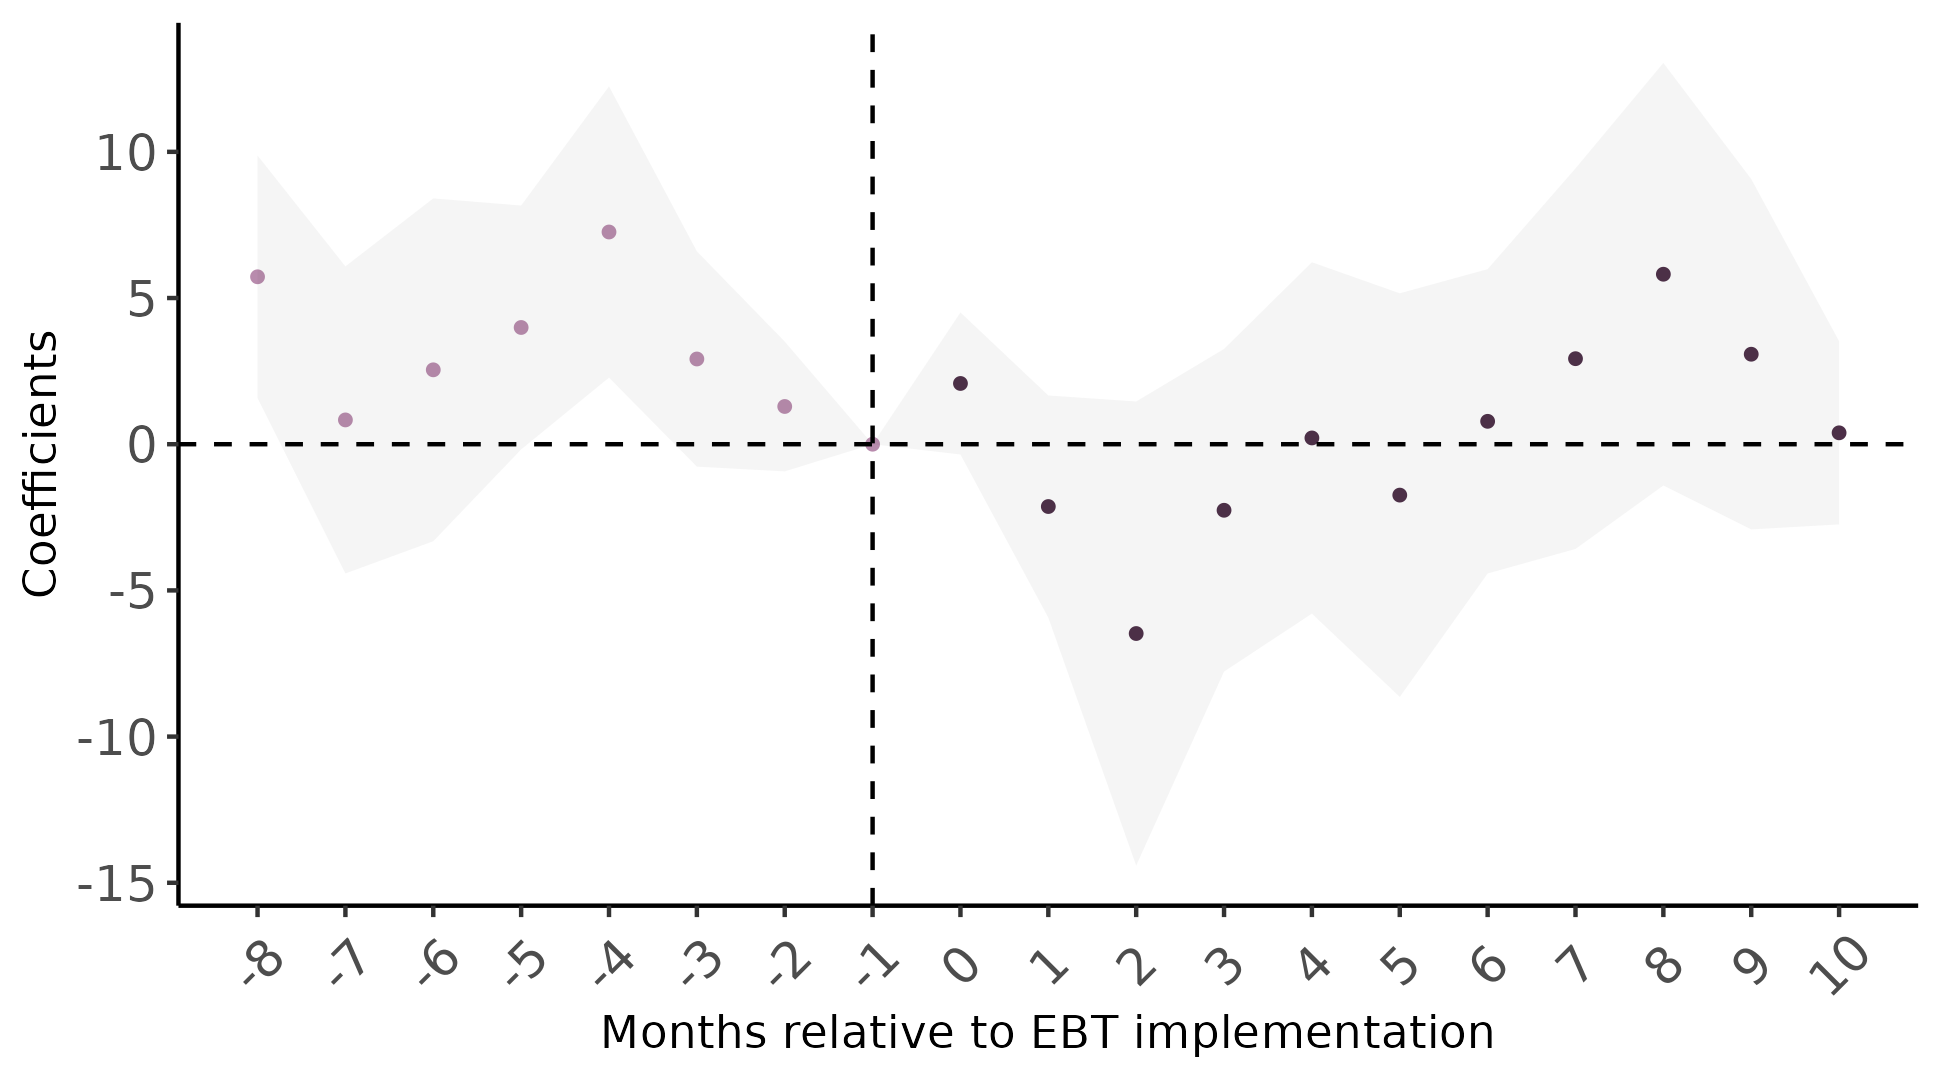
\includegraphics[width=\textwidth]{fig8_mk.png}  
		\caption{EBT and WIC Births per County (Figure 8 in \cite{meckel2020cure})}
		\label{mk_es1}
	\end{subfigure}
	\begin{subfigure}[t]{.5\textwidth}
		\centering
		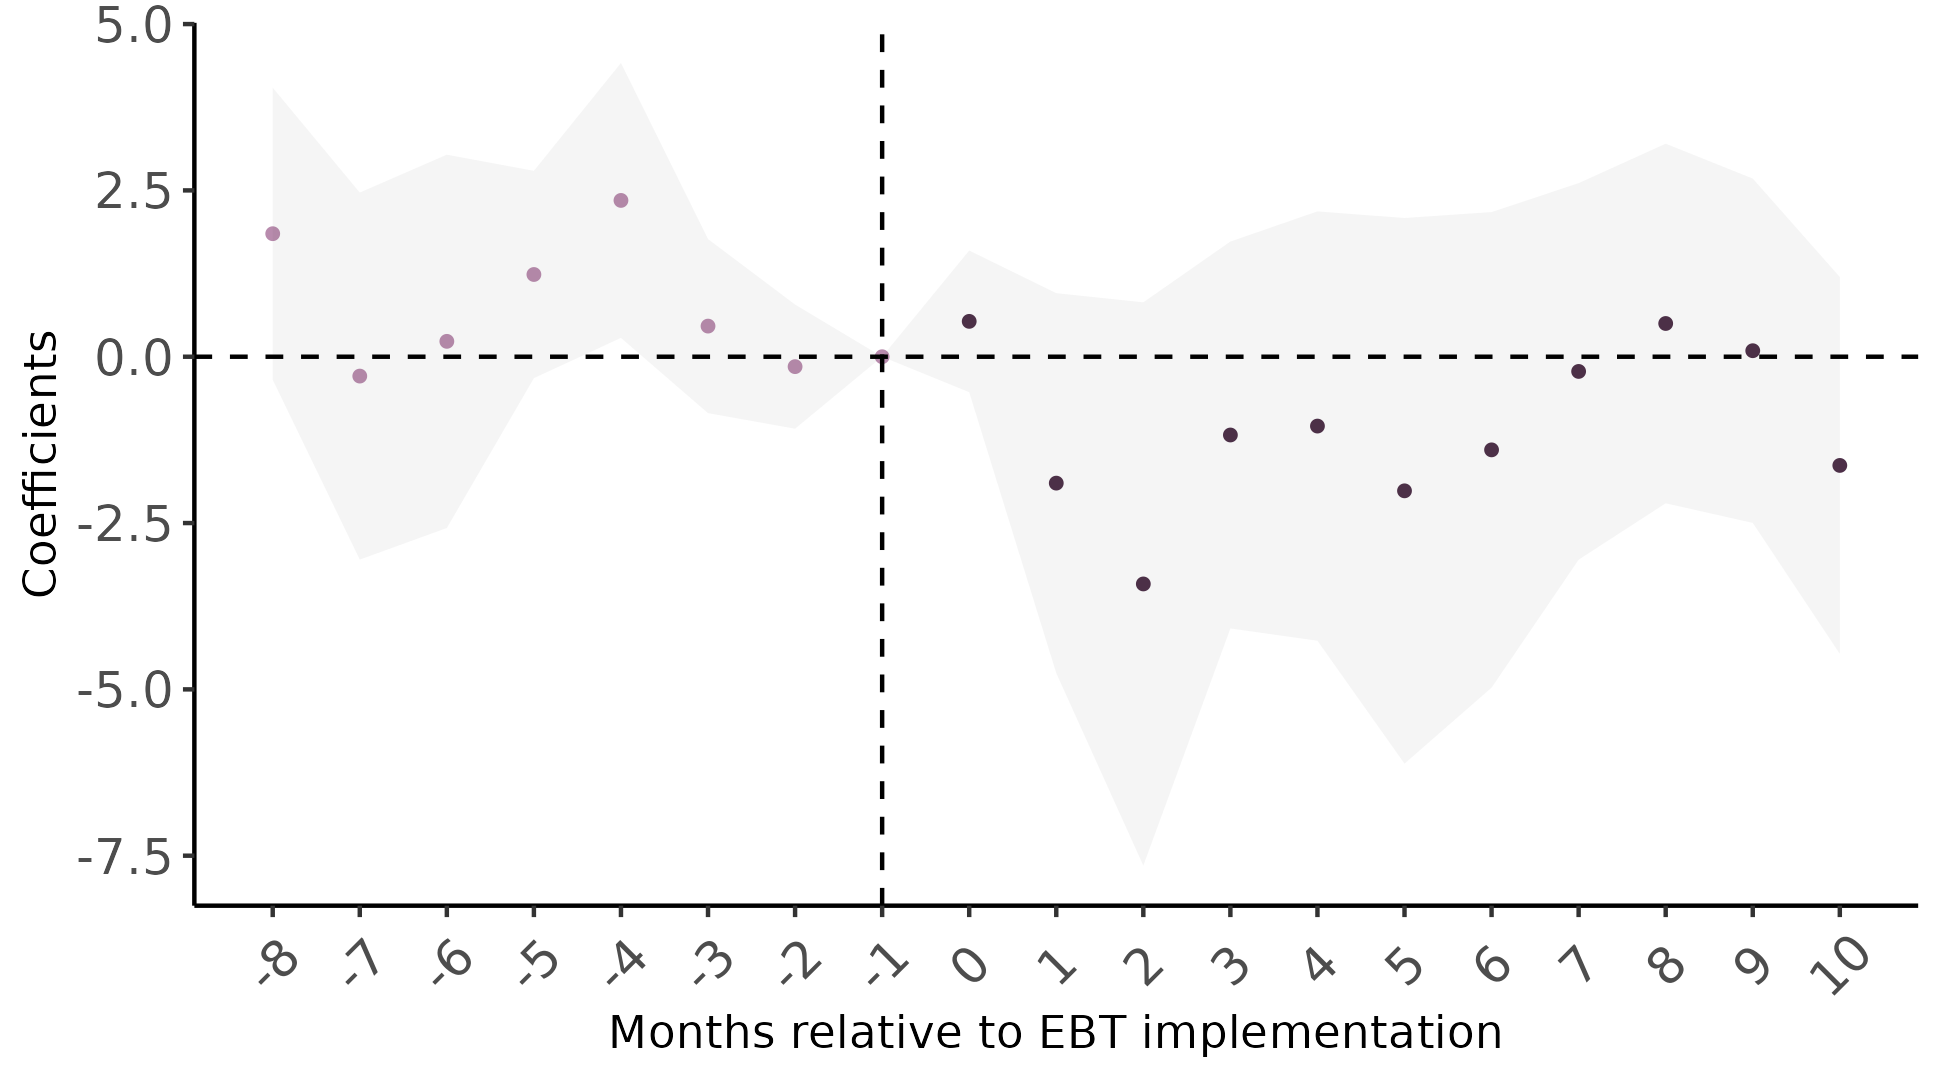
\includegraphics[width=\textwidth]{fig9_mk.png}  
		\caption{EBT and High Poverty WIC Births per County (Figure 8 in \cite{meckel2020cure})}
		\label{mk_es2}
	\end{subfigure}
	\begin{subfigure}[t]{.5\textwidth}
		\centering
		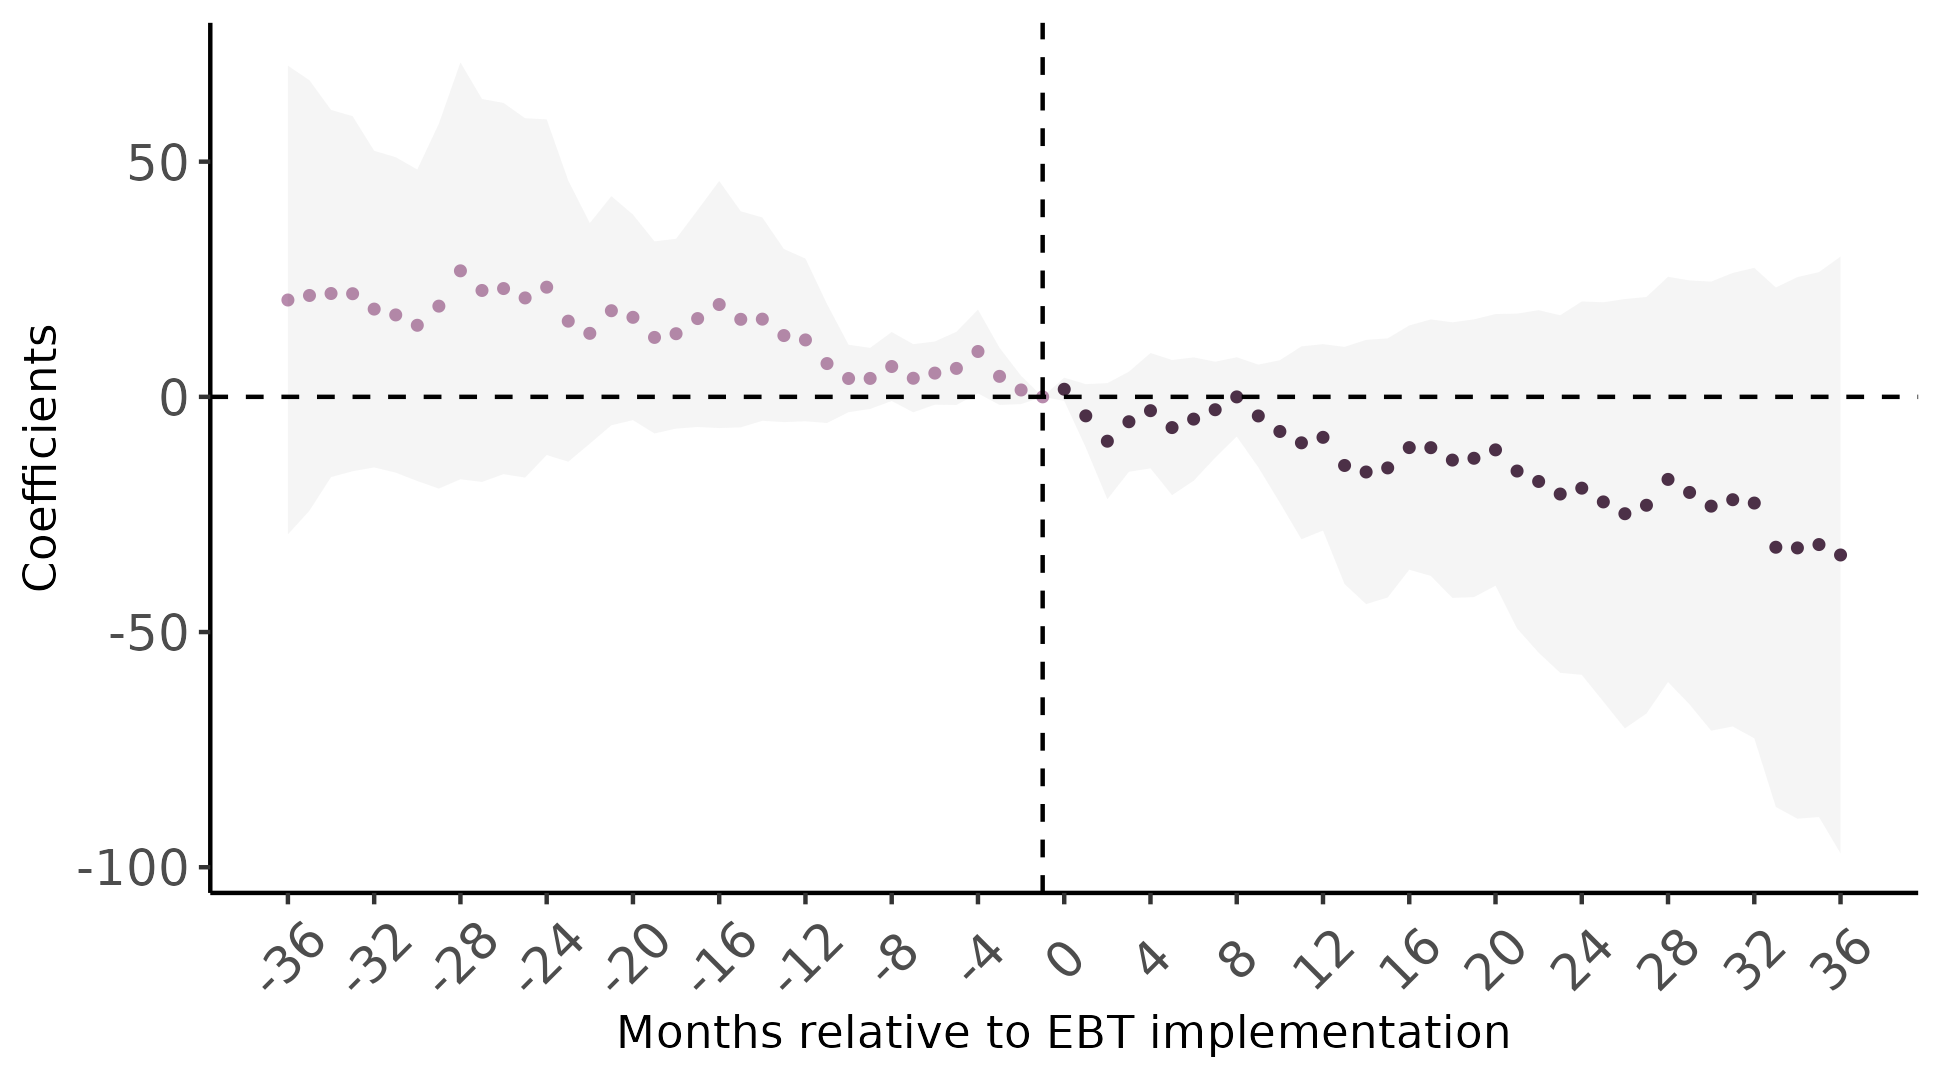
\includegraphics[width=\textwidth]{fig8_mk_long.png}  
		\caption{EBT and WIC Births per County, with A Larger Window}
		\label{mk_es3}
	\end{subfigure}
	\begin{subfigure}[t]{.5\textwidth}
		\centering
		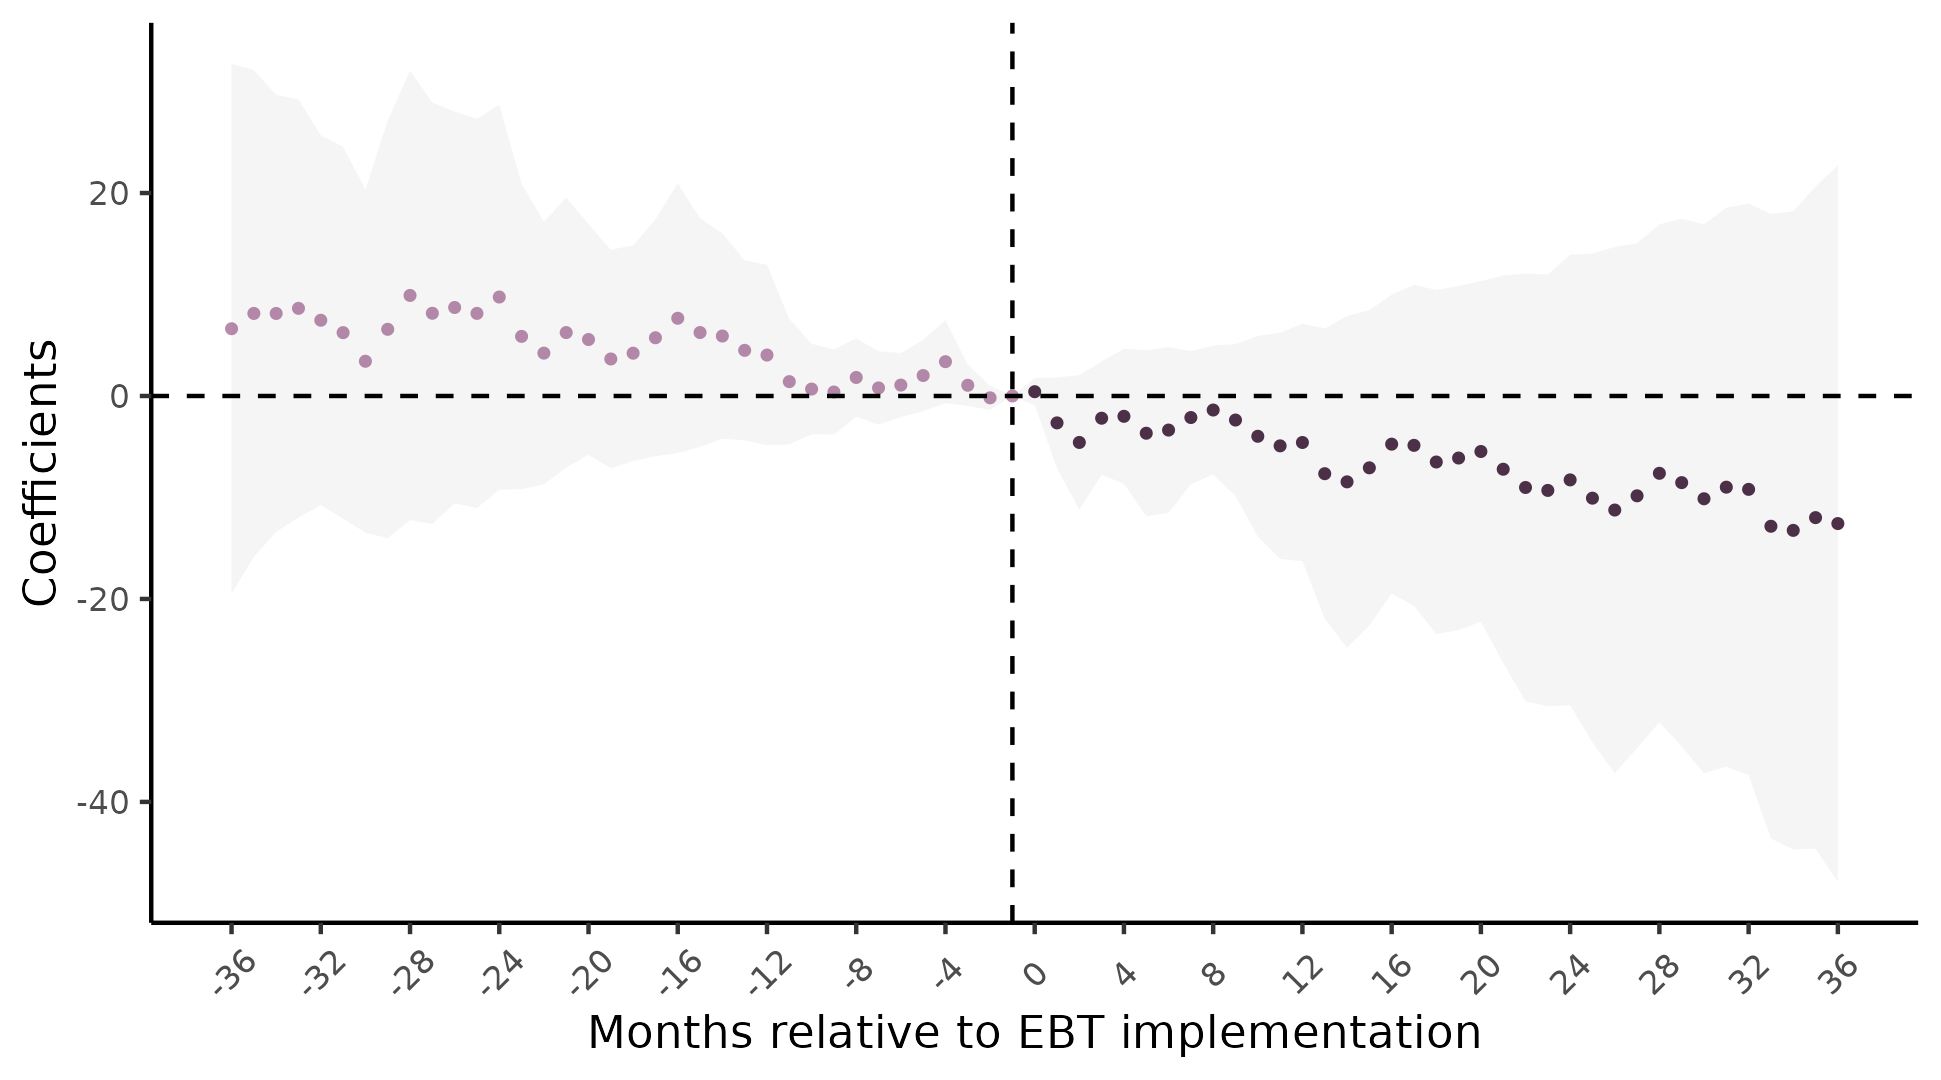
\includegraphics[width=\textwidth]{fig9_mk_long.png}  
		\caption{EBT and High Poverty WIC Births per County, with A Larger Window}
		\label{mk_es4}
	\end{subfigure}
	\caption{\textsc{Extending Event Study Plots in \cite{meckel2020cure} to A Larger Window}}
	\label{mk_es}
	\footnotesize
	\vspace{6pt}
	\vspace{4pt}
	Notes: 
\end{figure}


\begin{table}[!htbp]
	\begin{center}
		\caption{\textsc{Effects of EBT on WIC Births, Total Births, High Poverty Births, and High Poverty Births}} 
		\label{} 
		\scriptsize
		\begin{tabularx}{\linewidth}{@{}l*{8}{>{\centering\arraybackslash}X}@{}}
			\\[-1.8ex]\hline 
			\hline 
			\\[-1.8ex] 
			& \multicolumn{2}{c}{WIC Births} & \multicolumn{2}{c}{Total Births} & \multicolumn{2}{c}{High Poverty} & \multicolumn{2}{c}{High Poverty}  \\
			& \multicolumn{2}{c}{} & \multicolumn{2}{c}{} & \multicolumn{2}{c}{WIC Births} & \multicolumn{2}{c}{Births}  \\
			\cmidrule(lr){2-3}\cmidrule(lr){4-5} \cmidrule(lr){6-7}\cmidrule(lr){8-9}
			& (1)     & (2)      & (3)    & (4)  & (5)     & (6)      & (7)    & (8)    \\
			\midrule
			
			Born after EBT            & $-3.8563^{**}$ &                & $-3.9581^{**}$ &               & $-2.1681^{*}$ &                & $-1.9778^{**}$ &           \\
			& $(1.7398)$     &                & $(1.5992)$     &             & $(1.2410)$    &                & $(0.9566)$     &     \\
			Born 0-9 months &                & $-3.9151^{**}$ &                & $-3.7578^{**}$ &               & $-2.1380^{*}$  &                & $-1.9048^{**}$\\
			\hspace{8pt}    after EBT                       &                & $(1.8023)$     &                & $(1.5492)$     &               & $(1.2449)$     &                & $(0.9436)$    \\
			Born 10+ months  &                & $-3.2276^{**}$ &                & $-6.1000^{**}$  &               & $-2.4900^{**}$ &                & $-2.7591^{**}$ \\
			\hspace{8pt}    after EBT                &                & $(1.2863)$     &                & $(2.3564)$   &               & $(1.2604)$     &                & $(1.1791)$     \\
			\\
			R$^2$                     & $0.9893$       & $0.9893$       & $0.9961$       & $0.9961$    & $0.9854$      & $0.9854$       & $0.9923$       & $0.9923$     \\
			Observations                & $14,167$        & $14,167$        & $14,167$        & $14,167$    & $14,167$       & $14,167$        & $14,167$        & $14,167$      \\
			No. of Counties                & $239$          & $239$          & $239$          & $239$      & $239$         & $239$          & $239$          & $239$         \\  
			Dep. Var. Mean & $74.8541$ & $74.8541$ & $141.0398$ & $141.0398$ & $27.4343$ & $27.4343$ & $34.5791$ & $34.5791$  \\
			\hline \\[-1.8ex] 
			\hline 
			\hline \\ [-5.0ex] 		
		\end{tabularx}
	\end{center}
	\footnotesize
	\vspace{4pt}
	Notes: 
\end{table}

\begin{table}[!htbp]
	\begin{center}
		\caption{\textsc{Effects of EBT on WIC Birth Ratio and High Poverty WIC Birth Ratio}} 
		\label{} 
		\scriptsize
		\begin{tabularx}{.75\linewidth}{@{}l*{4}{>{\centering\arraybackslash}X}@{}}
			\\[-1.8ex]\hline 
			\hline 
			\\[-1.8ex] 
			& \multicolumn{2}{c}{WIC Birth Ratio} & \multicolumn{2}{c}{High Poverty} \\
			& \multicolumn{2}{c}{} & \multicolumn{2}{c}{WIC Birth Ratio} \\
			\cmidrule(lr){2-3}\cmidrule(lr){4-5}
			& (1)     & (2)      & (3)    & (4)    \\
			\midrule
			
			Born after EBT            & $-0.0153^{***}$ &                 & $-0.0218^{**}$ &                \\
			& $(0.0047)$      &                 & $(0.0088)$     &                \\
			Born 0-9 months after EBT &                 & $-0.0153^{***}$ &                & $-0.0219^{**}$ \\
			&                 & $(0.0046)$      &                & $(0.0088)$     \\
			Born 10+ months after EBT &                 & $-0.0175^{**}$  &                & $-0.0260$      \\
			&                 & $(0.0076)$      &                & $(0.0171)$     \\
			\\
			R$^2$                  & $0.8822$        & $0.8822$        & $0.4224$       & $0.4224$       \\
			Observations              & $14,167$         & $14,167$         & $12,286$        & $12,286$        \\
			Number of Counties              & $239$         & $239$          & $239$          & $239$          \\
			Dependent Variable Mean & $0.5606$ & $0.5606$ & $0.7870$ & $0.7870$ \\
			\hline \\[-1.8ex] 
			\hline 
			\hline \\ [-5.0ex] 		
		\end{tabularx}
	\end{center}
	\footnotesize
	\vspace{4pt}
	Notes: 
\end{table}

\begin{figure}[!htbp]
	\begin{subfigure}[t]{.5\textwidth}
		\centering
		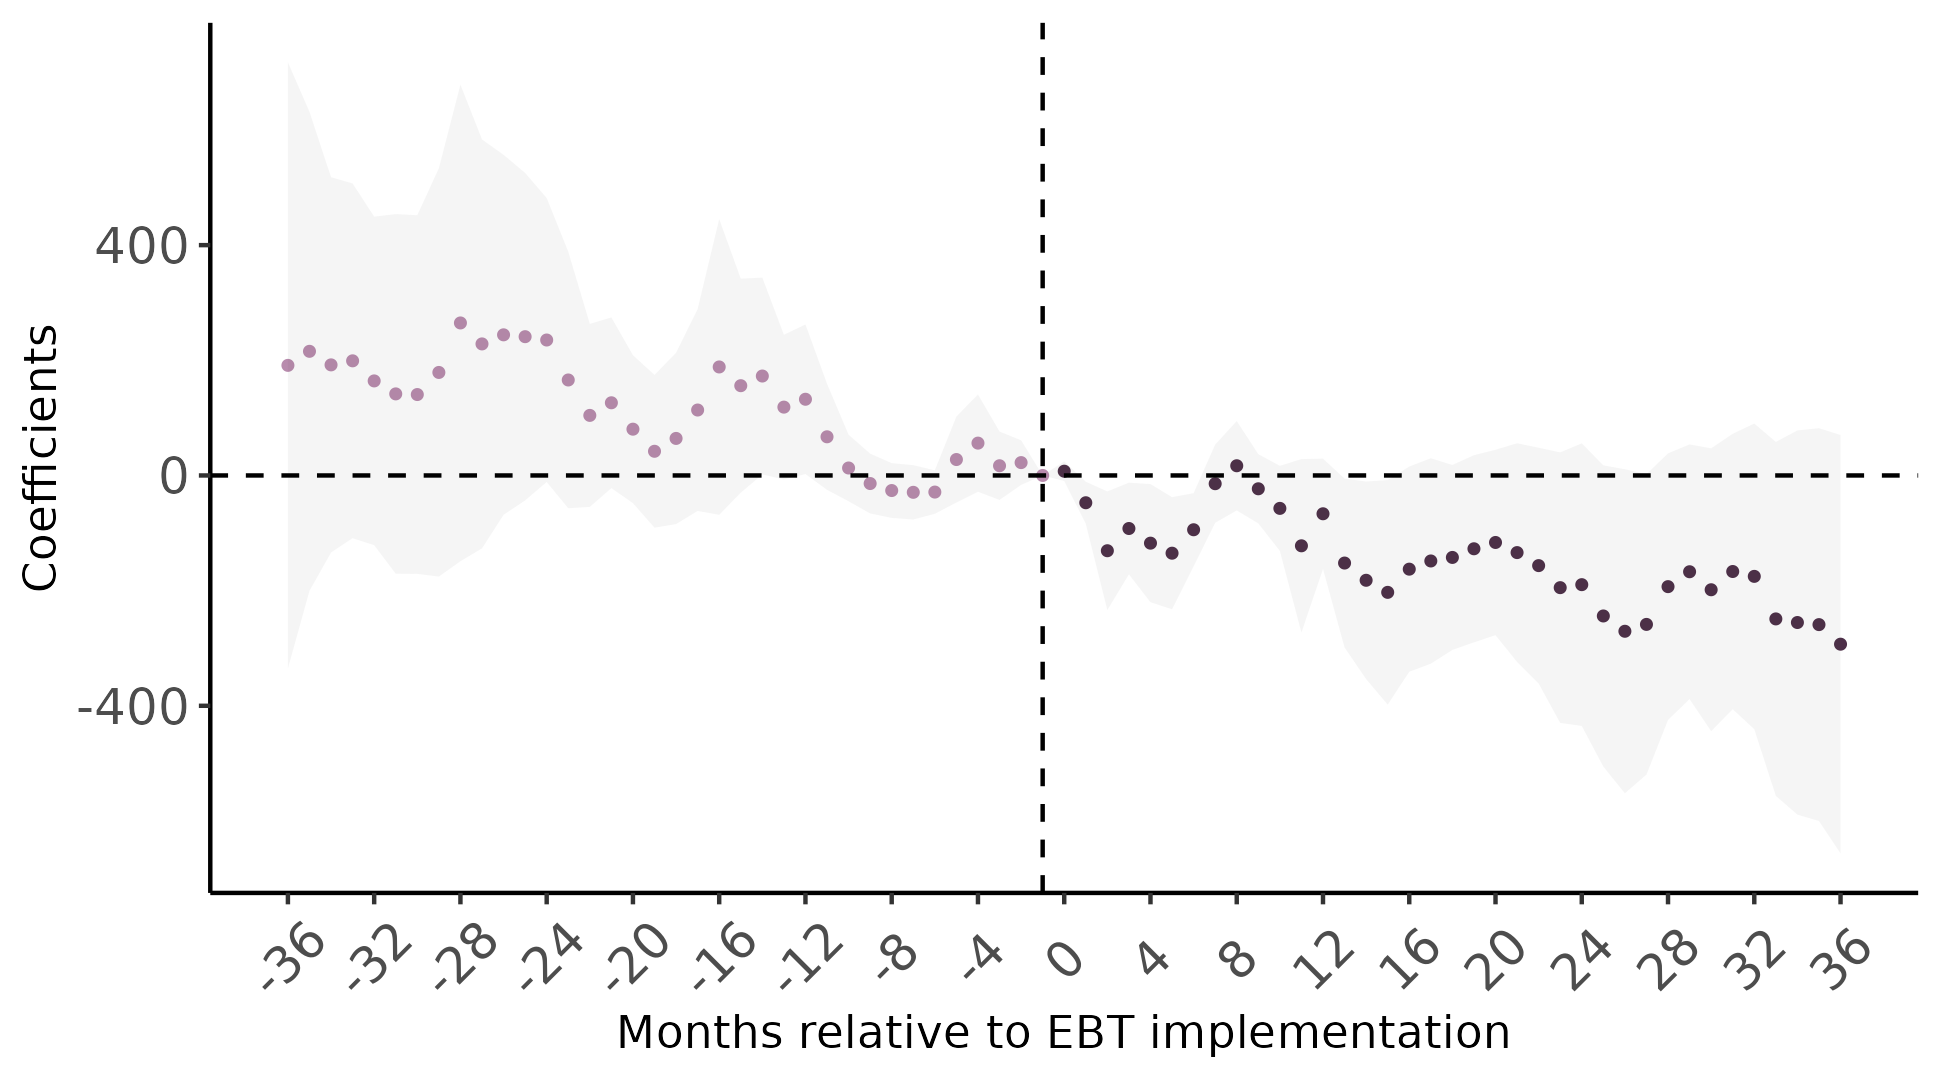
\includegraphics[width=\textwidth]{frac_mom_wic.png}  
		\caption{EBT and WIC Births Ratio}
		\label{mk_es1}
	\end{subfigure}
	\begin{subfigure}[t]{.5\textwidth}
		\centering
		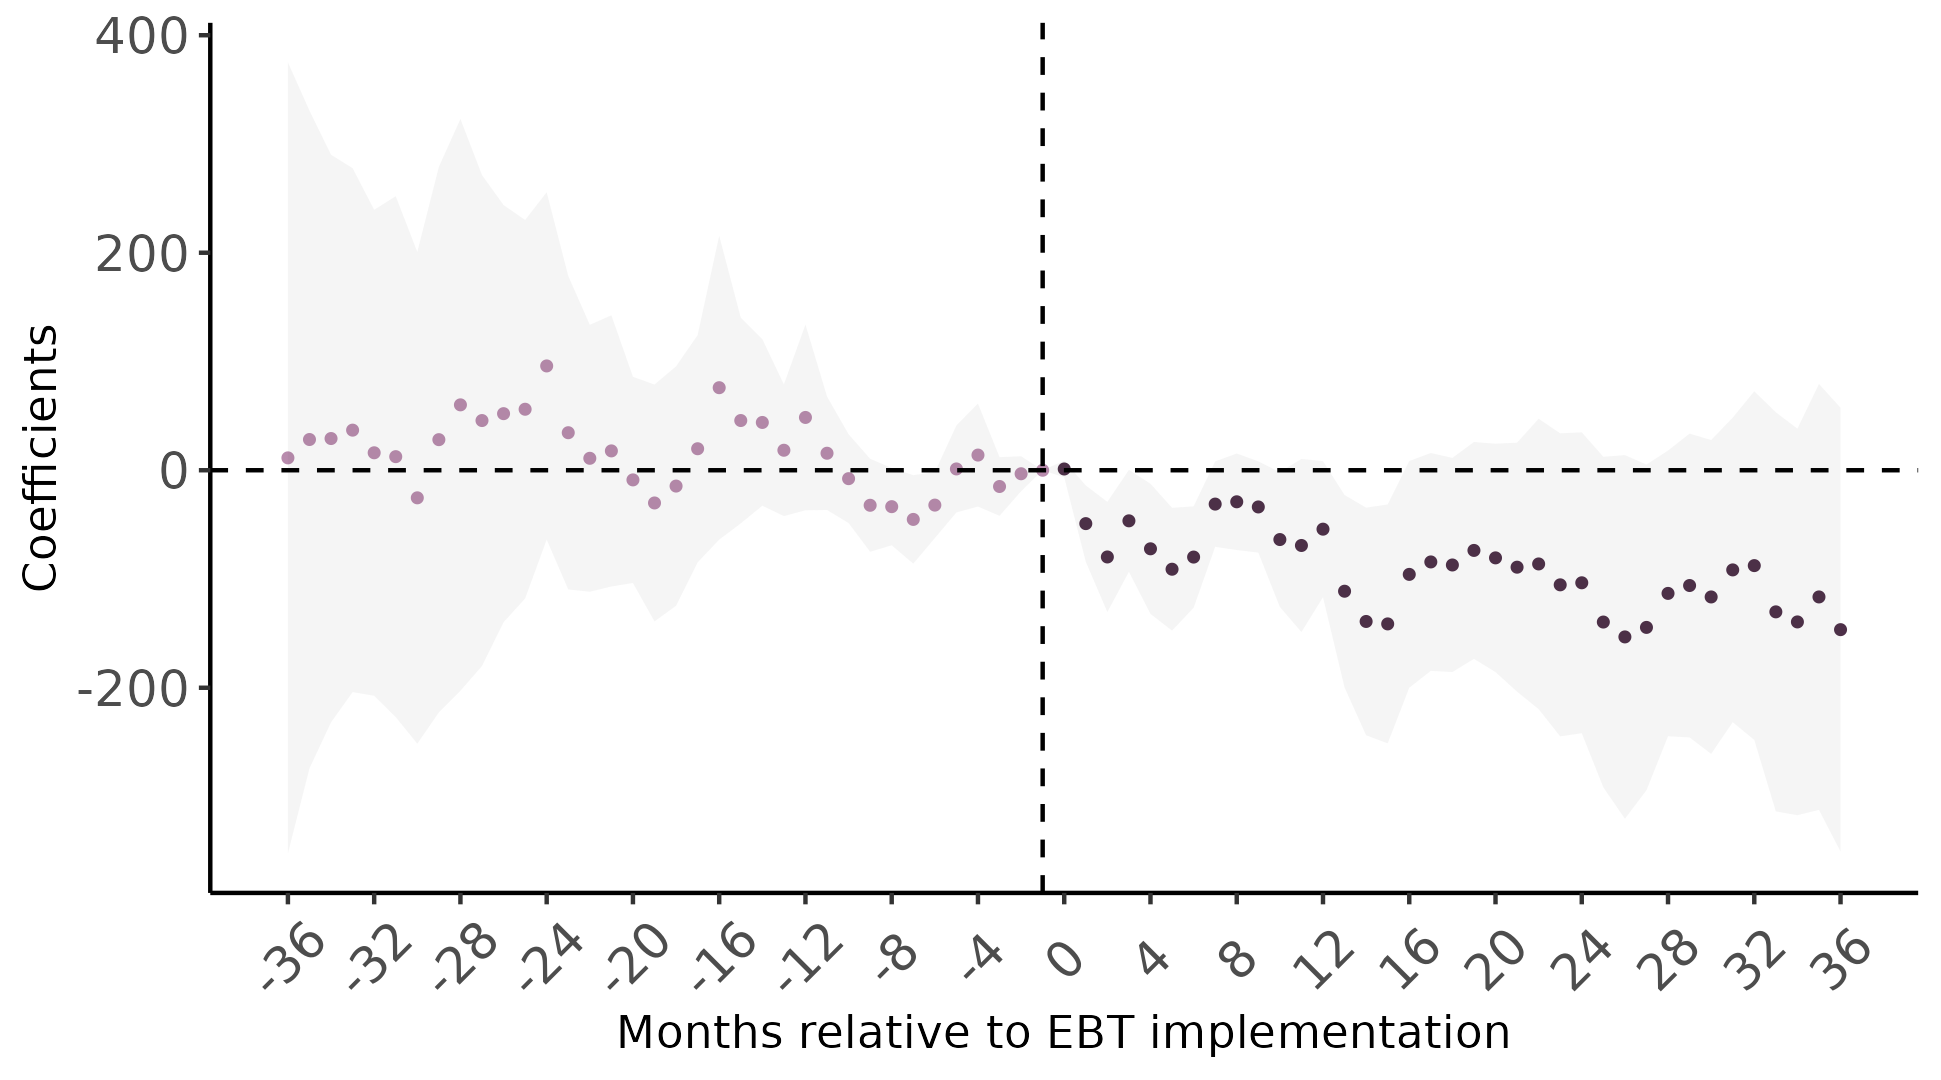
\includegraphics[width=\textwidth]{frac_poor_wic.png}  
		\caption{EBT and High Poverty WIC Birth Ratio}
		\label{mk_es2}
	\end{subfigure}
	\caption{\textsc{Event Study Plot for WIC Birth Ratio}}
	\label{mk_es}
	\footnotesize
	\vspace{6pt}
	\vspace{4pt}
	Notes: 
\end{figure}


\begin{table}[!htbp]
	\begin{center}
		\caption{\textsc{CS Estimators using Texas DSHS Data}} 
		\label{} 
		\scriptsize
		\begin{tabularx}{.9\linewidth}{@{}l*{6}{>{\centering\arraybackslash}X}@{}}
			\\[-1.8ex]\hline 
			\hline 
			\\[-1.8ex] 
			& \multicolumn{3}{c}{WIC Birth Ratio} & \multicolumn{3}{c}{High Poverty} \\
			& \multicolumn{3}{c}{} & \multicolumn{3}{c}{WIC Birth Ratio} \\
			\cmidrule(lr){2-4}\cmidrule(lr){5-7}
			& Full    & Full    & $\geq$ 15  &  Full    & Full    & $\geq$ 15  \\		
			& (1)     & (2)      & (3)    & (4)     & (5)    & (6)    \\
			\midrule
			
			Born after EBT  & -0.0102   &  -0.0297 & -0.0105  & -0.0067  &  -0.0446  &   0.0682$^{**}$   \\
			& (0.0069)  &  (0.0213) & (0.0319) & (0.0109) &  (0.0394)  &   (0.0283)   \\
			\\
			Covariates      &   &  \checkmark & \checkmark  &   &  \checkmark  &  \checkmark  \\
			Observations    & 10,050  & 10,050  & 5,200  &  5,750  &  5,750  &   4,350    \\
			Dep. Var. Mean (DVM)  & 0.5558  & 0.5558 &  0.5404 &  0.7935  &  0.7935  &   0.7960    \\
			\%(ATT/DVM)  &  -1.84\% &  -5.34\% &  -1.94\% & -0.84\%  &  -5.62\%  &   8.57\%   \\
			\hline \\[-1.8ex] 
			\hline 
			\hline \\ [-5.0ex] 		
		\end{tabularx}
	\end{center}
	\footnotesize
	\vspace{4pt}
	Notes: We report results with cells with more than 15 instead of 25 births to avoid having singular matrices.
\end{table}


\begin{figure}[!htbp]
	\begin{subfigure}[t]{.5\textwidth}
		\centering
		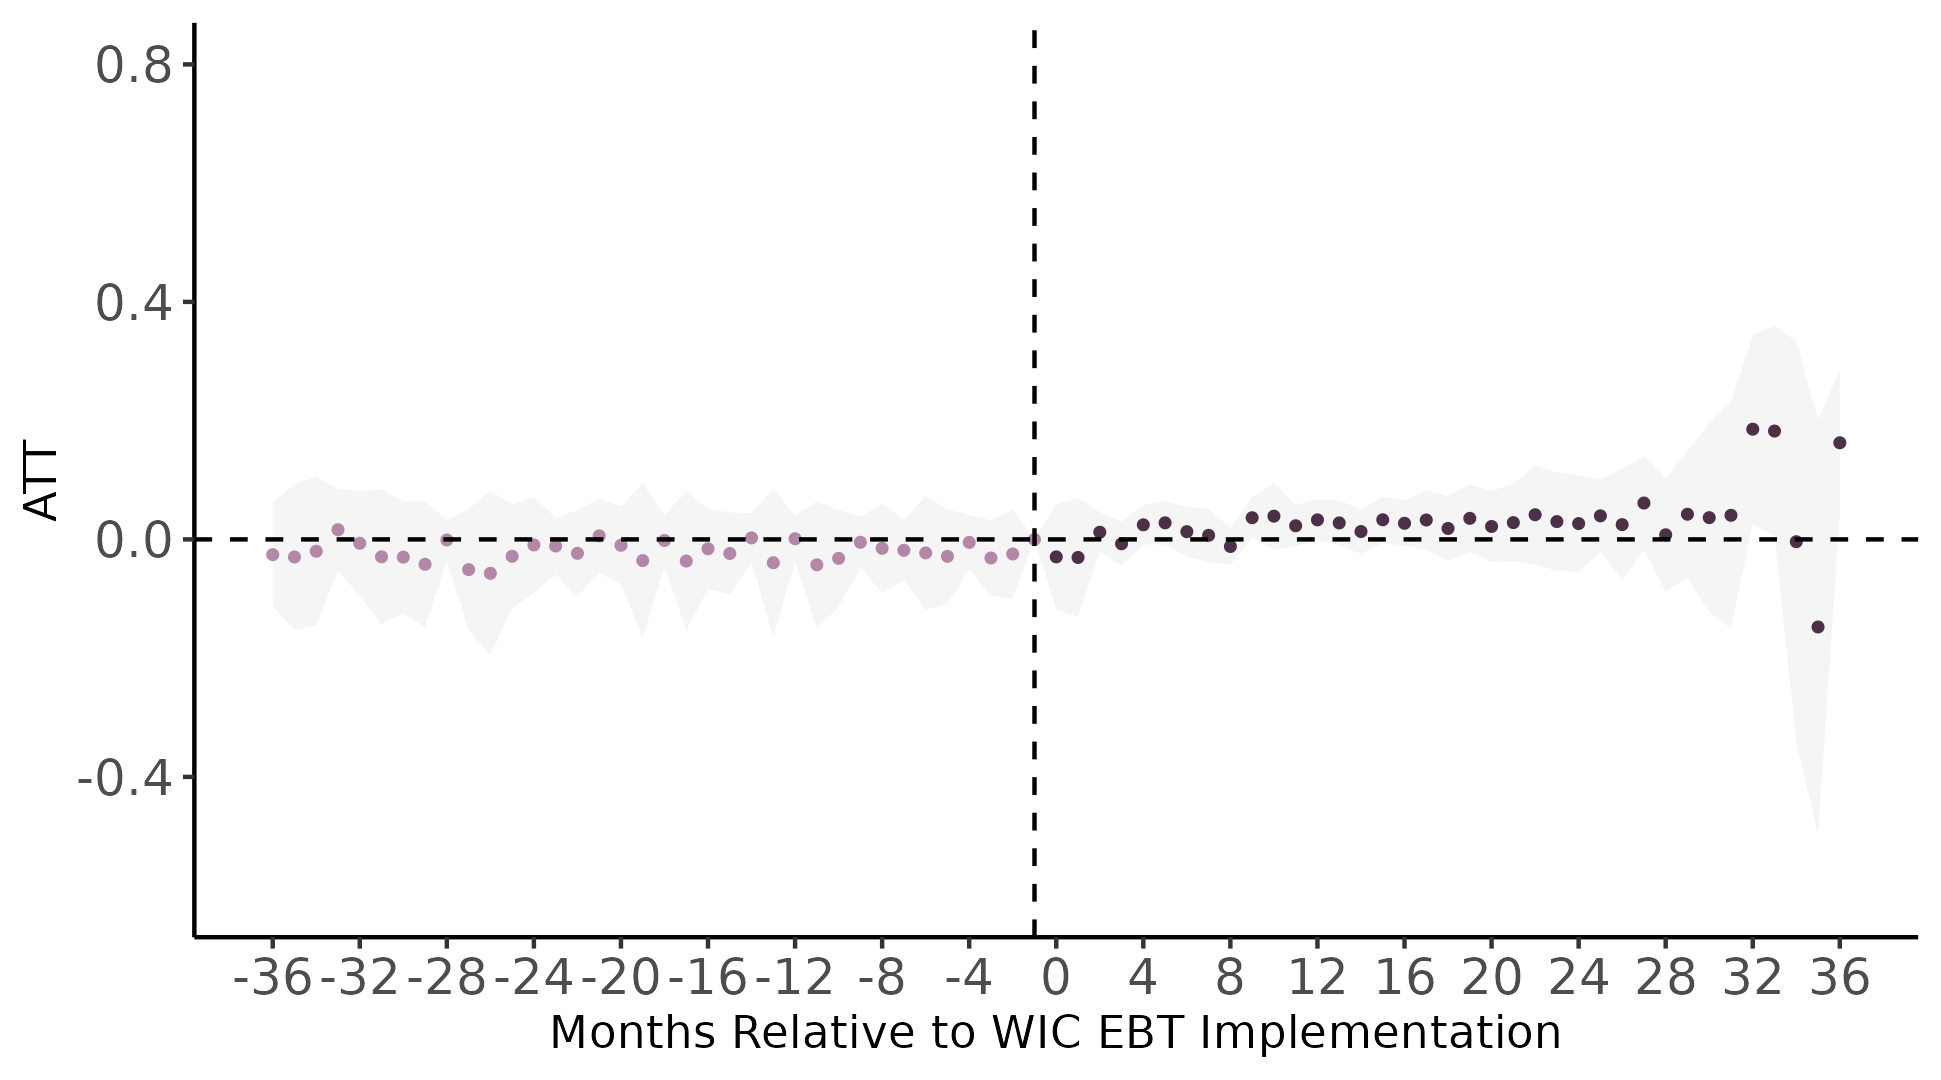
\includegraphics[width=\textwidth]{wic_tx_cs_es_frac_mom_wic.png}  
		\caption{WIC Births Ratio}
		\label{mk_es1}
	\end{subfigure}
	\begin{subfigure}[t]{.5\textwidth}
		\centering
		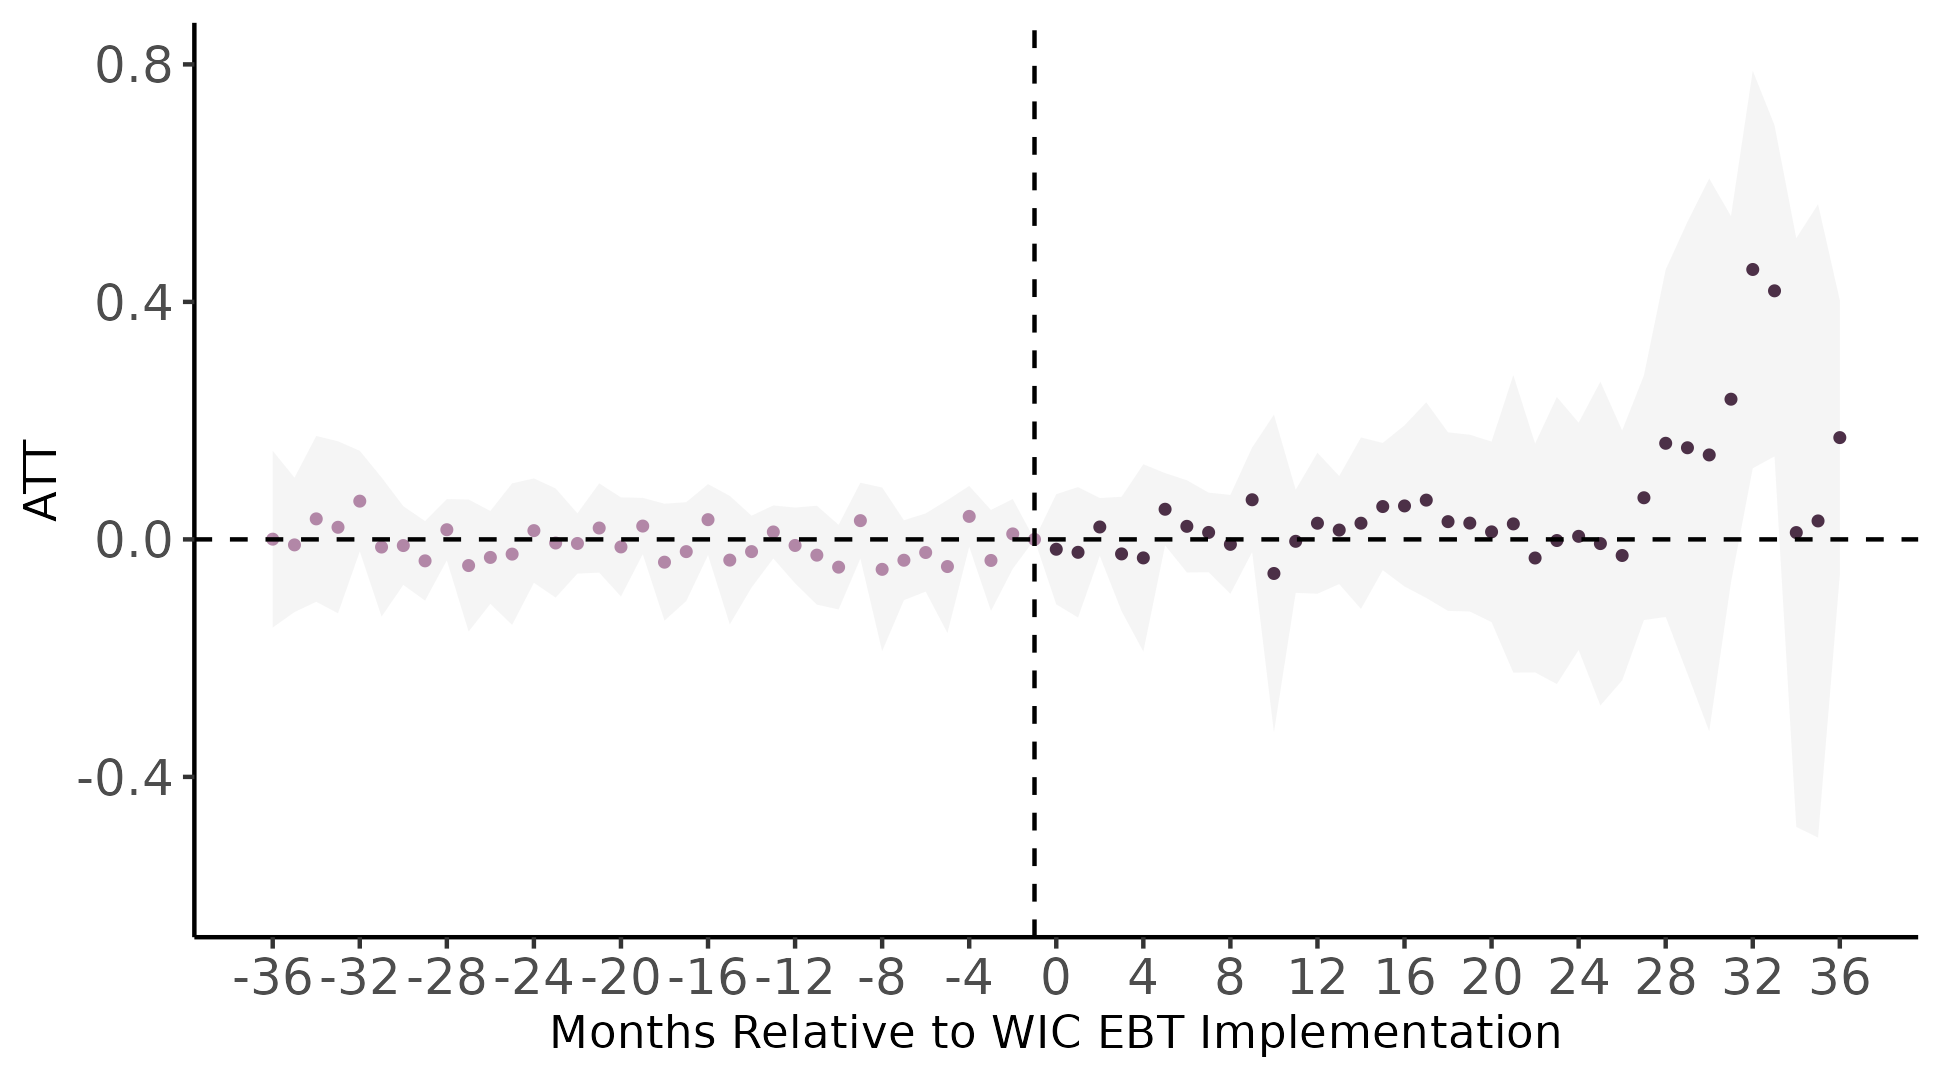
\includegraphics[width=\textwidth]{wic_tx_cs_es_frac_poor_wic.png}  
		\caption{High Poverty WIC Birth Ratio}
		\label{mk_es2}
	\end{subfigure}
	\caption{\textsc{Dynamic CS Estimates for WIC Birth Ratio}}
	\label{mk_es}
	\footnotesize
	\vspace{6pt}
	\vspace{4pt}
	Notes: As covariates we include all covariates from 2000 to 2004 as in our main results except income per person and net increase in WIC vendor due to unavailability of data. We replace income per person with median household income to account for baseline income difference.
\end{figure}
